
\documentclass[10pt,letterpaper]{article}
\usepackage[top=0.85in,left=0.85in,footskip=0.75in]{geometry}
% amsmath and amssymb packages, useful for mathematical formulas and symbols
\usepackage{amsmath,amssymb}
% Use adjustwidth environment to exceed column width (see example table in text)
\usepackage{changepage}
% Use Unicode characters when possible
\usepackage[utf8x]{inputenc}
% textcomp package and marvosym package for additional characters
\usepackage{textcomp,marvosym}
% cite package, to clean up citations in the main text. Do not remove.
\usepackage{cite}
\usepackage{url}
% Use nameref to cite supporting information files (see Supporting Information section for more info)
%\usepackage{nameref,hyperref}
% line numbers
%\usepackage[right]{lineno}

%\usepackage{natbib}
\usepackage{graphicx}
\usepackage{float}

% color can be used to apply background shading to table cells only
\usepackage[table]{xcolor}

% array package and thick rules for tables
\usepackage{array}
\usepackage{dsfont}

\usepackage{todonotes}
\usepackage{comment}

% referencing supplement-material
\usepackage{xr}
\externaldocument{./supplement}
%\usepackage{cleveref}



%% END MACROS SECTION

\title{Triqler for Protein Summarization of Data from Data Independent Aquisition Mass Spectrometry}
\author{Patrick Truong \and Matthew The \and Lukas K\"{a}ll}


\begin{document}
%\linenumbers
\maketitle

%Here I want to reference a figure that is in my supplementary content \cref{supp-fig:model_selection_criteria}.

%Here is a ref to the supplement, we have a Supplementary Figure \ref{fig:diff_vs_hela_find_a_better_label}.

\begin{abstract}

A frequent goal or subgoal when processing data from a quantitative shotgun proteomics experiment is a list of proteins that are differentially abundant under the examined experimental conditions. Unfortunately, obtaining such a list a challenging process, as the mass spectrometer analyses the proteolytic peptides of a protein, rather than the proteins themselves. We have previously designed a Bayesian hierarchical probabilistic model, Triqler, for combining peptide identification and quantification errors into probabilities of proteins being differentially abundant. 

Here we show that Triqler, is well compatible with data-independent acquisition data, despite being designed for data-dependent acquisition data. Furthermore, we find that it has better performance than other protein summarization tools when compared against a set of state-of-the-art DIA processing methods. 
\end{abstract}
  

\section*{Introduction}

Mass spectrometry (MS)-based proteomics enables efficient detection of proteins in complex mixtures. There are several different techniques to make the technology quantitative \cite{bantscheff2007quantitative,kall2011computational}, however, label-free quantification (LFQ) \cite{bondarenko2002identification} has an advantage in that it can handle larger sample sizes in a straight forward manner. For data from LFQ experiments, just as in other quantification schemes, there exists a plenthora of processing options, all containing several processing steps, each subject to their different error sources, all affecting the result of the processing.


We have previously designed a hierarchical Bayesian model, Triqler, able to control for errors from both the identification and quantification process in LFQ experiments\cite{The2018Integrated}. By integrating the error probabilities from identification and quantification one can obtain better accuracy in calling differentially abundant proteins. Triqler was designed for handling LFQ data from Data-dependent acquisition (DDA). However, many labs prefer Data-independent acquisition (DIA) mass spectrometry \cite{venable2004automated} as they find that it gives more reproducible peptide detection, and allow for a broader dynamical range in quantification \cite{bern2010deconvolution,zhang2020DIA}, compared to DDA. 

Here, we set out to investigate Triqler ability to summarize protein concentrations from peptide abundances derived from DIA data. We primarily used the LFQBench from Navarro et al. \cite{navarro2016multicenter} for the evaluation. In the original benchmark, Navarro et al. included a comparison of different protein summarization strategies and found that the so-called Top3 method generally resulted in lower variance and better quantification accuracy than the built-in methods from OpenSwath, SWATH2.0, Skyline, Spectronaut, and DIA-Umpire\cite{navarro2016multicenter}. However, there are reasons to believe that more sophisticated methods would yield better protein quantification than the Top3-method. Simple summarization methods based on mean and median peptide intensity have been shown to produce unreliable protein abundance estimates \cite{goeminne2015summarization}, and more advanced summarization strategies for LFQ data have been proposed in literature \cite{silva2006absolute,cox2014accurate}, and summarization techniques such as PQPQ~\cite{forshed2011enhanced}, MSstats~\cite{choi2014msstats}, Diffacto~\cite{zhang2017covariation}, MSqRob2~\cite{sticker2020robust} and Triqler~\cite{The2018Integrated} has all been shown to outperform Top3 and there currently exists no reason why stated methods would not theoretically be able to perform well for DIA data. Hence, we found it apt to benchmark Triqler against a set of state-of-the-art protein summarization methods using peptide quantities from the LFQBench DIA data set.
 
 
\section*{Materials and methods}


\subsection*{Data description}
\subsubsection*{LFQBench mass spectrometry data}


We downloaded the LFQBench dataset~\cite{navarro2016multicenter} from PRIDE identifier PXD002952. Here we used the TripleTOF6600 section of the study, which was harvested with a setup of 32 fixed windows MS2-windows. We also restricted ourselves to the low ratio difference samples, referred to as the HYE124 hybrid proteome samples in the original study. That consists of triplicates of Sample A composed of tryptically digested proteins from 65\% w/w HeLa, 30\% w/w yeast, and 5\% w/w \textit{E. coli} cells, and triplicates of Sample B, composed of 65\% w/w, 15\% w/w yeast, and 20\% w/w \textit{E. coli} proteins. Samples from HYE110 and the TripleTOF5600 section of PXD002952 were omitted in this study. Further details about mass spectrometric instrumentation and data acquisition are available in Navarro et al.~\cite{navarro2016multicenter}. The \verb|.wiff| files were converted to \verb|.mzML| files in a centroided format using msconvert (using windows OS msconvert version 3.0) with peakPicking filter msLevel=1-). 


\subsubsection*{LFQBench sequence database}

Uniprot FASTA files with one protein sequence per gene were downloaded for each species (UP000005640, UP000000625, and UP000002311, acquired on 2021-06-16). The unfiltered FASTA files contained 20 590 human proteins, 6 046 yeast proteins, and 4 373 \textit{E. coli} proteins. To reduce the effect of the different protein inference strategies for the tested protein summarization tools, a modified FASTA file, without shared peptides, was used for database search. The filter randomly removed protein sequences with shared peptides, so that the final database did not contain any tryptic peptides with length $>$7 amino acids mapping to peptides shared with other proteins. After filtering the FASTA file contained 20 302 proteins (288 human proteins fewer proteins than an unfiltered database), 5 848 yeast proteins (198 yeast proteins fewer proteins than an unfiltered database), and 4 306 \textit{E. Coli} proteins (67 \textit{E. Coli} proteins than unfiltered database). Replacing the I/L amino acids to handle mass-equivalence did not result in any considerable differences (See Supplementary Table \ref{table:proteins_in_database}). We also added pseudo-reverse sequences to the database as decoys for target-decoy analysis using OpenSwathDecoyGenerator. 


\subsubsection*{Biological study data}
We downloaded a dataset containing quantitative proteomic analysis of oxaliplatin(OXA) induced peripheral neurotoxicity \cite{YANG2022104682} referred here as the OXA-dataset from PRIDE identifier PXD031322. The OXA-dataset consist of DIA mass-spectrometry data of three groups; control (Ctrl), 1 week post OXA injection called short-term(ST) and 2 weeks post OXA injection called long-term(LT). The Ctrl group contains 5 samples, the ST group contains 5 samples and the LT group contains 4 samples. The OXA-dataset also contains a set of gas phase fragmentation (GPF) DIA mass spectrometry data which were used to for spectral library generation in by Yang et al. For this part of the study we used the supplied spectral library from the data repository. Further details about the mass spectrometry instrumentation and data acquisition are available in Yang et al. \cite{YANG2022104682}.   

\subsection*{General workflow}

We used two separate strategies to generate peptide abundances from the DIA-runs. First, we used a spectral library consisting of selected spectra from separate DDA runs, we refer to this workflow as ID hereon, and secondly, we searched pseudo-spectra generated directly from the DIA data, we will refer to this workflow as PS from hereon. The workflows are shown in Figure \ref{fig:flowchart}. We will describe the parameter choices of both these two methods below.

\begin{figure}[htp]
    \centering
    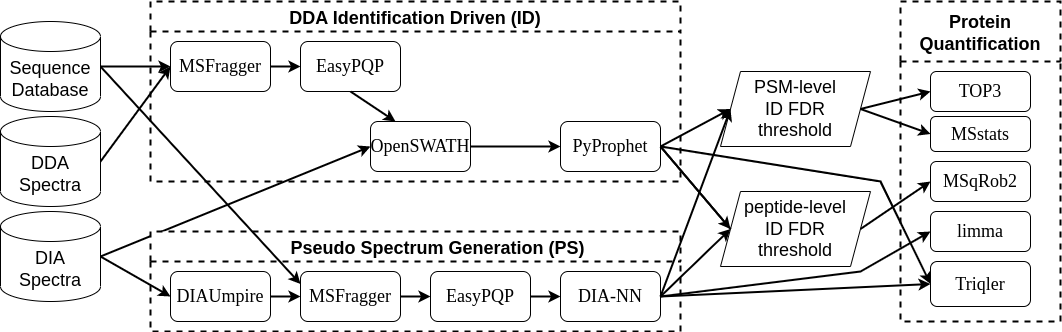
\includegraphics[width=1.0\linewidth]{./img/methods.png} 
    \caption{{\bf The DDA identification-driven matching (ID) and pseudo spectrum workflow pipelines (PS).} In the pipelines DIA-Umpire(SE), MSFragger and EasyPQP is run from Fragpipe (\protect\url{https://fragpipe.nesvilab.org/}). Identification thresholds of 1\% on PSM-level was applied for Top3 and MSstats, and peptide-level for MSqRob2, while the identifications were provided unfiltered to Triqler. \label{fig:flowchart}}      
\end{figure}



\subsubsection*{DDA identification-driven (ID) spectral library}

For the ID workflow, we searched the LFQBench provided DDA runs with MSFragger\cite{kong2017msfragger} with default settings (Precursor mass tolerance of [-20, 20] ppms, fragment tolerance of 20 ppms, Calibration and Optimization: ``Max calibration, parameter optimization'', isotope error: 0/1, Data type: DDA, Load rules: stricttrypsin, Cut after: KR, Cleavages: ENZYMATIC, Missed cleavages: 2, Clip N-term M: True, Peptide length of [7, 50], Peptide mass range of [500, 5000], Split database: 1, and allowing for oxidation on methionine and protein N-terminus modifier as variable modifications), and a spectral library was constructed with EasyPQP \cite{easypqp} with the default setting (RT Calibration: ``Automatic selection of a run as reference RT'', RT Lowess Fraction: 0.1, UniMod annotation tol(Da), Fragment annotation tol(ppm): 15, and the default PSM-level threshold of 0.01, peptide-level false discovery rate (FDR) of 0.01, and protein-level FDR of 0.01). OpenSwatchDecoyGenerator was used to generate decoys for the spectral library with a pseudo-reverse method. The DIA data searched with the spectral library through OpenSwath Workflow, and an \texttt{m\_score} computed using PyProphet\cite{teleman2015diana}. An \texttt{m\_score} cut-off for a user-specified peptide identification false-discovery rate is computed with SWATH2STATS \cite{blattmann2016swath2stats}. This process resulted in a set of detected peptides together with their assessed peptide identification accuracies and abundance estimates (Supplementary Table \ref{fig:osw_peptide_and_protein_id} shows the number of identified peptides and proteins).


\subsubsection*{Pseudo Spectra generation (PS) spectral library}

For the PS workflow we also used the fragpipe software, employing DIA-Umpire to extract pseudo-spectra from the DIA data. The DIA-Umpire parameters was set to default values (MS1 PPM: 10, MS2 PPM: 20, Max Missed Scans: 1, Mass Defect Filter: True, RP max: 25, RF max: 500, Corr Treshold: 0, Delta Apex: 0.2, RT Overlap 0.3, Mass Defect Offset 0.1, Isotope Pattern: 0.3, MS1 SN: 1.1, MS2 SN: 1.1, Adjust Fragment Intensity: True). The pseudo-spectra were subsequently searched using using MSFragger with default settings (Precursor mass tolerance of [-20, 20] ppms, fragment tolerance of 20 ppms, Calibration and Optimization: ``Max calibration, parameter optimization'', isotope error: 0/1, Data type: DDA, Load rules: stricttrypsin, Cut after: KR, Cleavages: ENZYMATIC, Missed cleavages: 2, Clip N-term M: True, Peptide length of [7, 50], Peptide mass range of [500, 5000], Split database: 1, and allowing for oxidation on methionine and protein N-terminus modifier as variable modifications). A spectral library was build from the resulting PSMs using easyPQP with default setting (RT Calibration: ``Automatic selection of a run as reference RT'', RT Lowess Fraction: 0.1, UniMod annotation tol(Da), Fragment annotation tol(ppm): 15, and the default PSM-level treshold of 0.01, peptide-level FDR of 0.01, and protein-level FDR of 0.01). DIA-NN was used for peptide quantifications with settings specified in \url{https://fragpipe.nesvilab.org/docs/tutorial_DIA.html#quantify-with-dia-nn} (Protein inference: ``Off'', Quantification strategy: ``Robust LC (High accuracy)'', Precursor FDR (\%): 1.0, Protease: ``Trypsin/P'', Missed cleavages: 1, Maximum number of cariable modifications: 0, N-term M excision: True, C carbamidomethylation: True, Peptide length: [7, 30], Precursor m/z range: [300, 1800], Fragment ion m/z range: [200, 1800], Mass accuracy: 0.0, MS1 accuracy: 0.0, Scan window: 0, Use isotopologues: True, Remove likely interferences: True, Neural network classifier: ``Single-pass mode'', Protein inference: Genes, Cross-run normalization: ``RT-dependent'', Library generation: ``Smart profiling''). Too compute false discover rates DIA-NN uses a built-in custom implementation of the mProphet algorithm\cite{reiter2011mprophet, demichev2020dia} (Supplementary Table \ref{fig:diann_peptide_and_protein_id} shows the number of identified peptides and proteins). 
 
\subsection*{Protein summarization}

The peptide quantities were summarized to proteins using the average of the three most intense peptides (We call it Top3), MSstats, MSqRob2, and Triqler. This is done for both the ID and PS pipelines. 

\subsubsection*{Top3}

We implemented a short script that take the average of the 3 most abundant PSMs for each protein and sample. In samples only having two PSMs these were also included, still represented by their average. Proteins with one or zero PSMs per sample were excluded . PSMs were filtered at an 1\% PSM-level FDR before performing the Top3 protein summarization. 

\subsubsection*{MSstats}

We installed MSstats version 3.18.5 using R/Bioconductor (available at \url{https://www.bioconductor.org/packages/release/bioc/html/MSstats.html}). MSstats use feature-level data, allowing for multiple PSM hits per peptide identification. We filtered so that every protein had at least 2 peptides and a maximum of 10 peptides, and we thresholded with a \texttt{m\_score} which corresponds to a peptide identification FDR lower than 0.01 for both ID and PS pipelines. In the PS pipeline, the data was filtered on the \texttt{Q.Value} columns from the DIA-NN output file. In the ID pipeline we computed an \texttt{m\_score} corresponding to an 1\% FDR and used this \texttt{m\_score} to filter the data. MSstats was run using the MSstats command \texttt{dataProcess}. The significance testing between conditions was performed using the MSstats function \texttt{groupComparison}.  

\subsubsection*{MSqRob2}
%
We installed MSqRob2 version 0.9 using R/Bioconductor (available at \url{https://github.com/statOmics/msqrob2}). MSqRob2 takes peptide-level input. The output from OpenSwath and DIA-NN is at PSM-level. We select the top PSM hit as our peptide and filter the data on 1\% peptide level FDR to get peptide-level data. The highest scoring PSMs are selected by the highest \texttt{m\_score} for OpenSwath and highest \texttt{CScore} for DIA-NN. MsqRob2 was run using the MSqRob2 command \texttt{msqrob},  contrast was set to \texttt{condition}.
MSqRob2 uses \texttt{lme4} to construct a linear-mixed model with random effect, but without fixed effect. The models specified in by the variable formulas the constructs the models $y = Z_1 \mu + \epsilon$ and $y = Z_2 \mu + \epsilon$, where $Z_1$ contains the random effects condition, sample and feature (peptides for protein) and $Z_2$ contains only a random effect for condition. Some proteins have only intensities from one peptide. This can cause the first model $y = Z_1 \mu + \epsilon$ parameters to fail to converge. For these proteins we use the reduced model $y = Z_2 \mu + \epsilon$.
%clear
\subsubsection*{Triqler}

We downloaded Triqler from \url{https://github.com/statisticalbiotechnology/triqler}. We used Triqler v0.6.1 for the tests described in this paper. We selected a lower bound estimate for the \texttt{fold\_change\_eval} parameter as described in The\&K\"{a}ll \cite{the2021triqler}, which ended up as 0.76 for the spectral library data, and 0.51 for the pseudo-spectra enabled data.

As Triqler's model accounts for the assessed uncertainty in the prior identification steps of the data, it does not threshold the PSMs but instead takes all of the PSMs as input. The \texttt{searchScore} column should reflect increasing certainty in PSMs. Therefore we apply negative log-transform to the \texttt{m\_score} or \texttt{Q.Value} to indicate \texttt{searchScore} for the two different pipelines. 

\subsubsection*{Multiple Hypothesis Correction}
There was a slight difference in some of the benchmarking metrics, as the multiple test correction is performed with $q$~value for Triqler and Top3, while MsStats and MSqRob2 use Benjamini-Hochberger \cite{benjamini1995controlling} corrections. The $q$~value approach aims to give an unbiased estimator of FDR, while the Benjamini-Hochberger approach estimates the upper bound of the FDR (and will therefore result in an FDR equal to or higher than the $q$~value). As a consequence, the statistics from MSstats and MSqRob2 should be more conservative than the estimates from Triqler and Top3\cite{korthauer2019practical}.


\subsection*{Application to real biological data}
To show that our results are relevant for real biological application we reanalyse the OXA-dataset. We group the data as in Yang et al. \cite{YANG2022104682}. The proteins in cluster 1(C1) and 2(C2) were continually up-regulated or down-regulated from Ctrl to ST and from ST to LT. The proteins in cluster 3(C3) and 4(C4) were proteins up-regulated or down-regulated from ST to LT, and the proteins in cluster 5(C5) and 6(C6) were up-regulated or down-regulated from Ctrl to ST.  

\section*{Results}

To establish that Triqler is useful when evaluating DIA data, we first examined the DIA data to establish that the abundance values derived from such processes are in line with the assumptions that Triqler makes about input data, and second we benchmarked Triqler against a set of state-of-the-art methods for protein summarization. For both tasks, we used selected parts of the LFQBench dataset, which we processed in two different ways. We used a pipeline with a DDA identification-driven (ID) spectral library, as well as one using a Pseudo Spectra generation (PS) spectral library (See Methods).


\subsection*{Validations of properties of DIA peptide abundance}

DIA data is assumed to encompass a larger dynamic range than DDA data \citation{bilbao2015processing}. This could affect one of Triqler's assumptions, that the noise structure is mainly multiplicative, i.e. that the standard deviation within a sample group is proportional to its mean. When investigating all the peptide abundance measurements at a 1\% PSM identification false discovery rate (FDR) from the TripleTOF6600 section of the LFQBench dataset, we found a relatively linear relationship between standard deviation and mean (Supplementary Figure \ref{fig:uniform_offset_in_standard_deviation_boxplot}A-D). Further, Triqler assumes that the missing peptide abundance values follow a censored normal distribution, which is also roughly fulfilled by DIA data (See Supplementary Figure \ref{fig:fraction_missing_values}).


\subsection*{Harmonization of protein inference procedures.}

Encouraged by the finding that peptide abundances from DIA data have similar properties to those of DDA data, we wanted to see how well Triqler works in practice. Particularly, we wanted to compare the performance of Triqler to that of other protein summarization methods. However, to do so we first needed to establish some principles for how to benchmark summarization methods on data from whole-cell mixtures, when comparing methods that use different protein inference procedures \cite{serang2012recognizing}. When reporting the number of differentially abundant proteins in data sets from mixtures from whole-cell extracts, a protein inference scheme that infers any protein containing a detected peptide will report more differentially abundant proteins than a more restrictive scheme that just reports a parsimonious set of proteins. There are no restrictive mechanisms detecting situations where non-present proteoforms are reported as long as they are reported with protein abundance rates compatible with the right proteome. To alleviate, or at least minimize, this problem from our comparison, we restricted the searched sequence database by removing proteins with shared peptides. This operation strived to give a fairer comparison of protein summarization regardless of the protein inference method.

To filter the database file to a single sequence per protein database, we implemented a script that splits all the protein sequences before lysine (K) and arginine (R). For these amino acids. If the sequences are shorter than 7 amino acids, we select the one amino acid sequence per protein at random to keep and discard the rest. 

\subsubsection*{Distributions of the estimated fold changes}

Triqler is not meant as a tool to give point estimates of abundances, instead triqler is suited for calculating distributions of protein fold changes. However, to make a usefull comparison to other methods, one can use the Triqler's maximum a posteriors (MAPs) as point estimates of protein abundance. 

We applied Triqler, MSstats, MSqRob2, and Top3(see the Methods section) to the peptide abundances derived from the ID and PS workflows from the varying concentrations of {\em E. Coli} and yeast concentrations in a background of HeLa-cells of the LFQBench set. As a first overview of the results we made histograms of  Triqler's protein-level fold change MAPs as well as the compared methods estimated fold-changes (Figure \ref{fig:fc_histogram}). For the comparison removed the methods' fold change selection mechanisms.

Triqler and Top3 appears to have less fold-change bias than MSstats and MSqRob2, that is, the apex of the distributions is centered more closely to the lysate mixture rates. MSstats and MSqRob2 have distribution apexes that for each species that are centered at lower fold changes than the true lysate mixture rates. Reprocessing the data with replaced labels led to the reversed result, i.e. the apxeses centered around values higher that the pipetted mixture rates for both MSstats and MSqRob2 (data not shown).  We also observe that the apex of the distributions has higher values for Triqler than the other methods. We also observe in Figure \ref{fig:fc_scatter} that the regression line goes towards the true fold-change values for Triqler, while it remains constantly postive for Top3, MSstats and MSqRob2. We also observe that Triqler has longer tails for the estimated yeast and {\em E. Coli} fold change distributions. These values are explained by proteins quantified with fewer peptides, i.e. less certain protein quantification. It appears as the proteins with correctly estimated foldchanges are identified by more peptides that the one off from their expected fold change, as can be seen in in Figure \ref{fig:number_of_peptides_supplement}, which show the number of peptides per protein for different Triqler estimated fold changes.


\begin{figure}[hbt]
    \centering
    \begin{tabular}{cc}
	    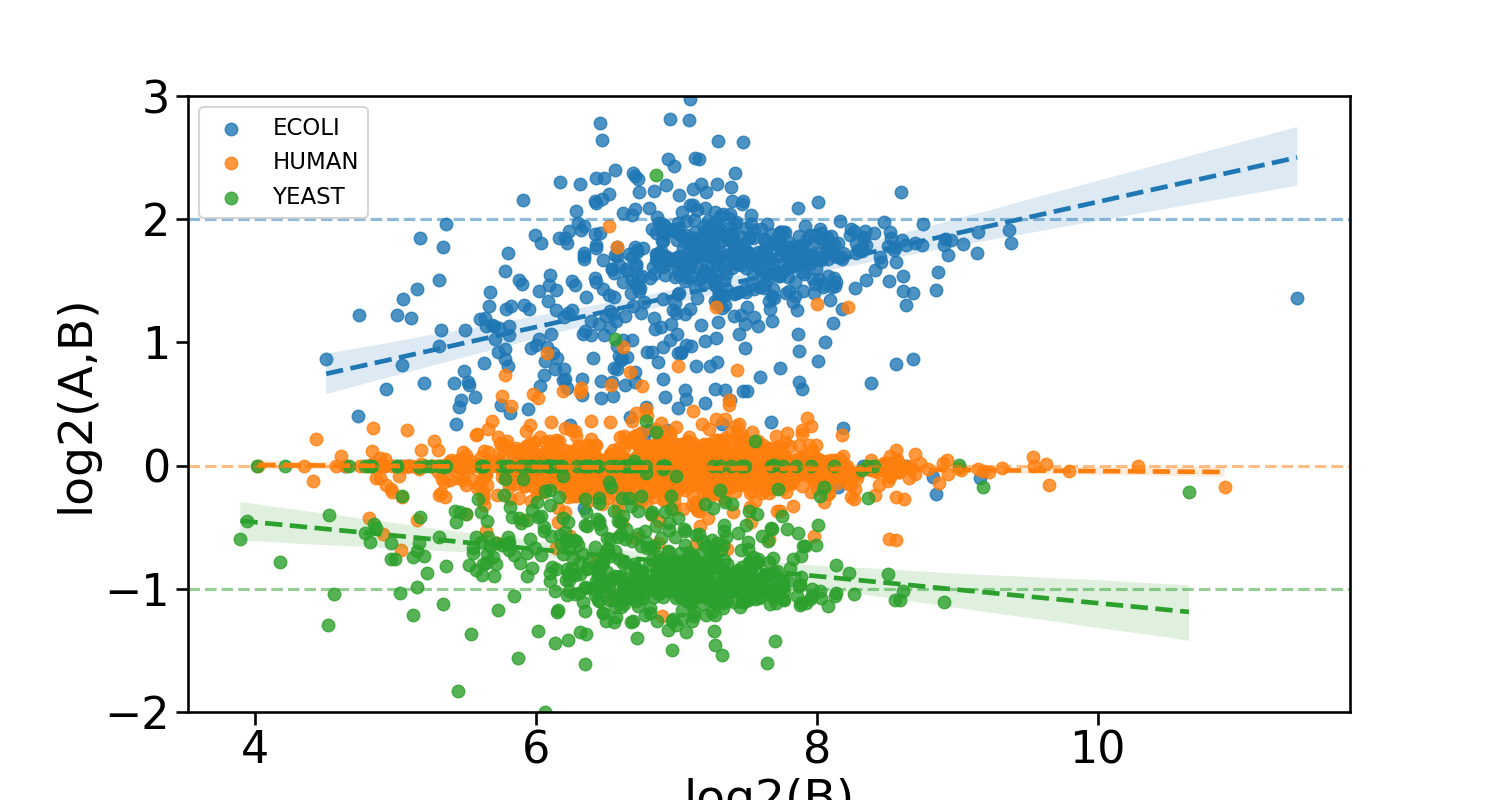
\includegraphics[width=0.45\linewidth]{../../result/report_plots_pipeline/scatter_ID_triqler.png} & 
	    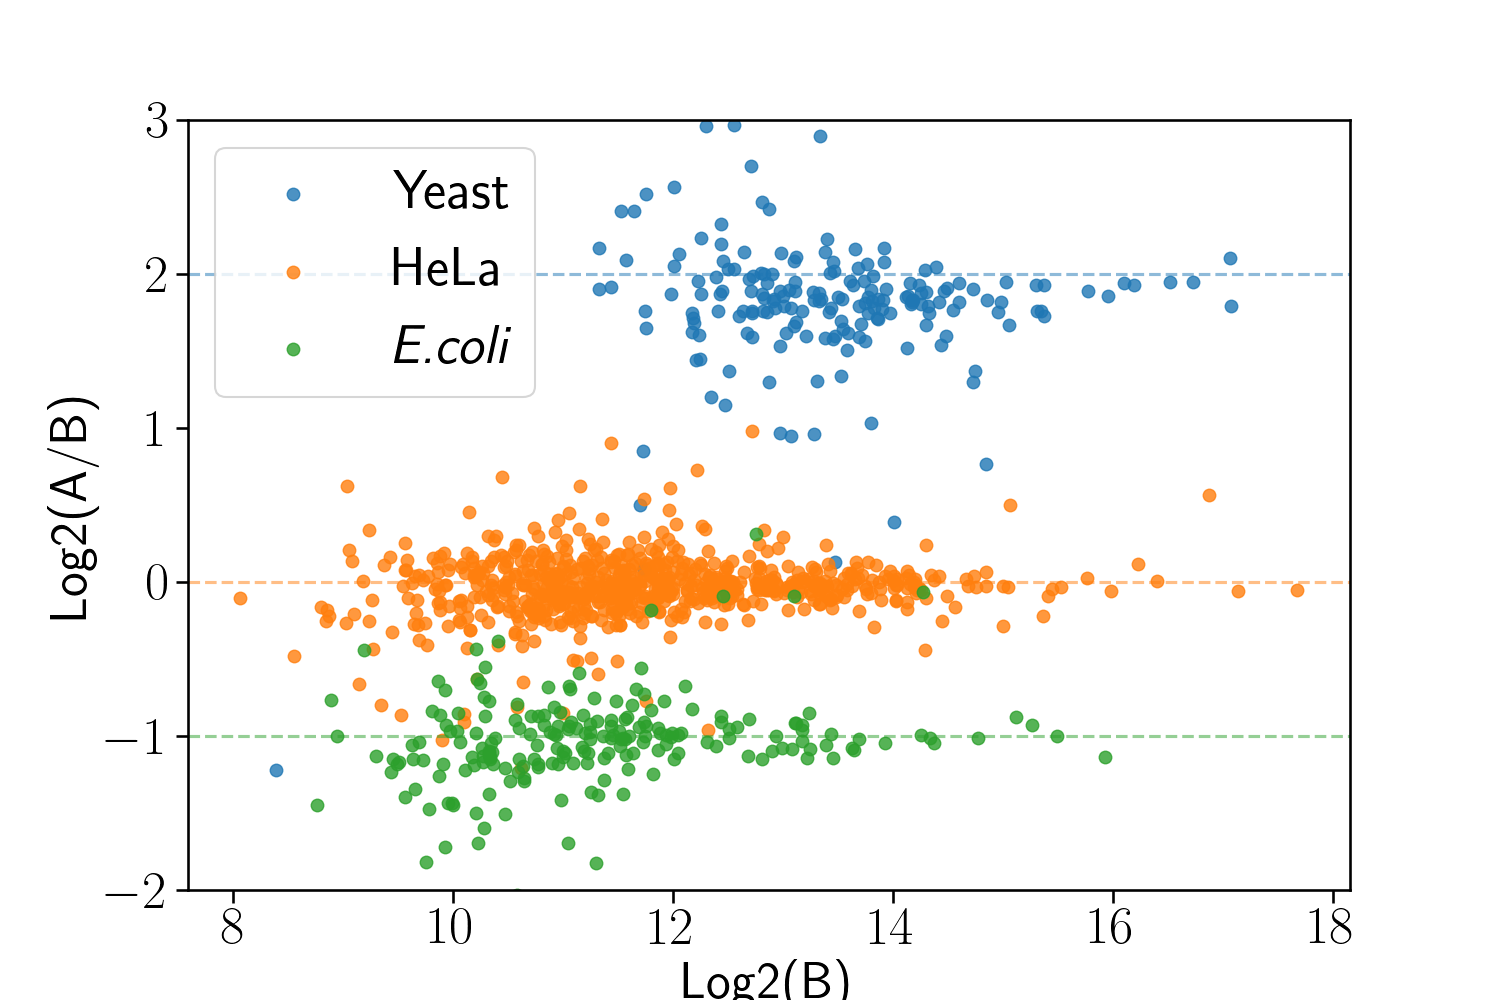
\includegraphics[width=0.45\linewidth]{../../result/report_plots_pipeline/scatter_ID_top3.png} \\ 
        A & B \\ 
	    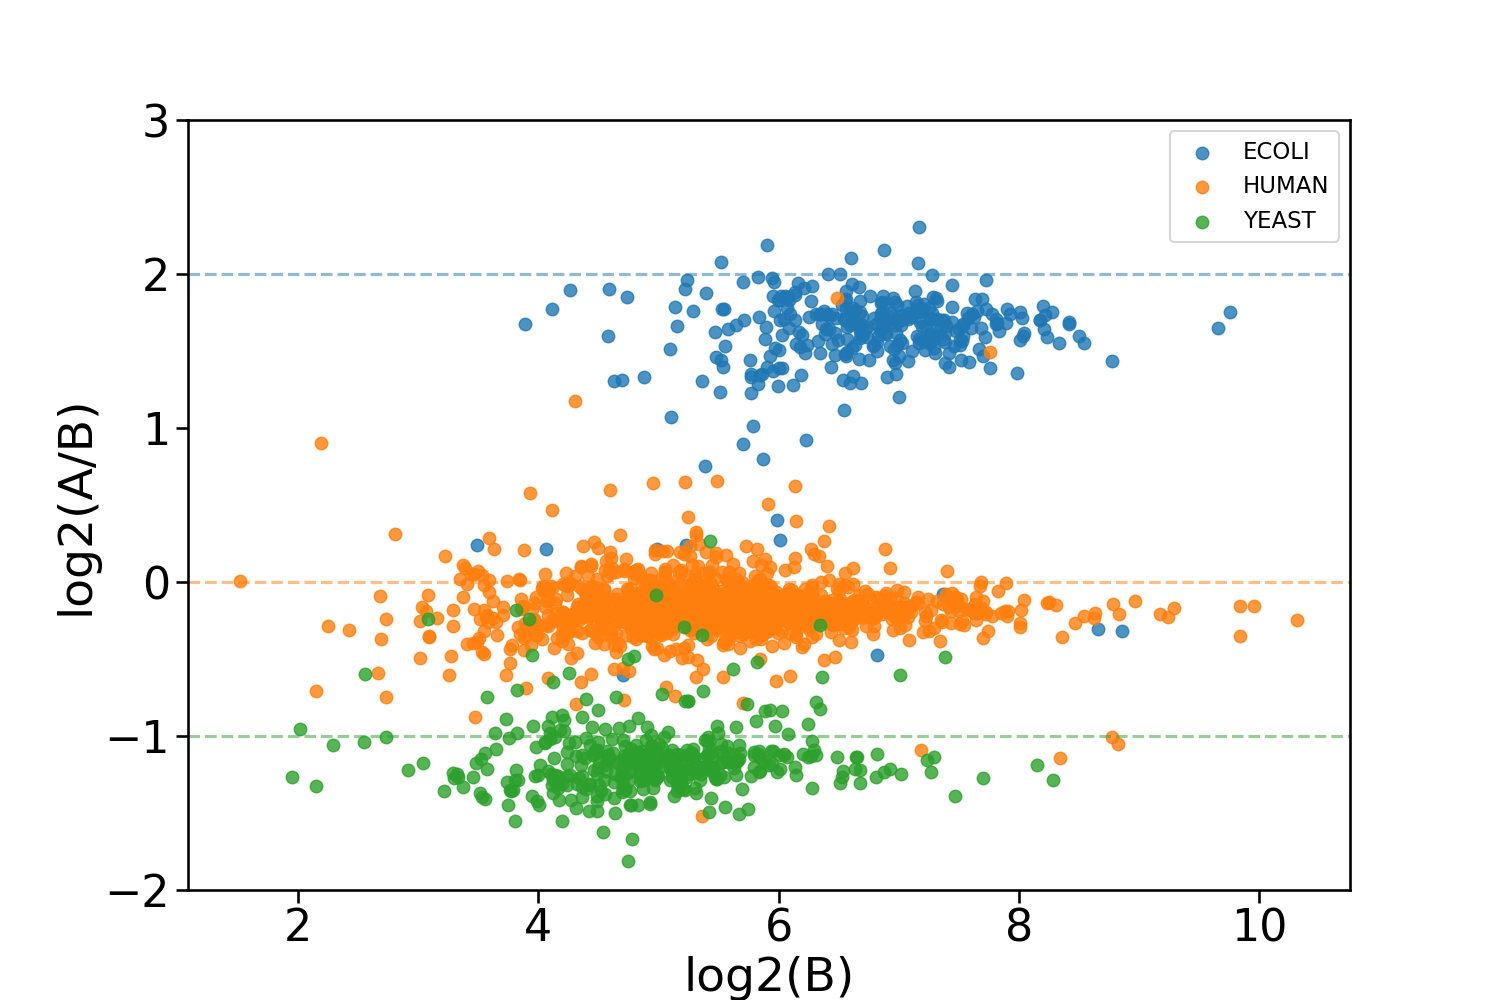
\includegraphics[width=0.45\linewidth]{../../result/report_plots_pipeline/scatter_ID_msstats.png} & 
	    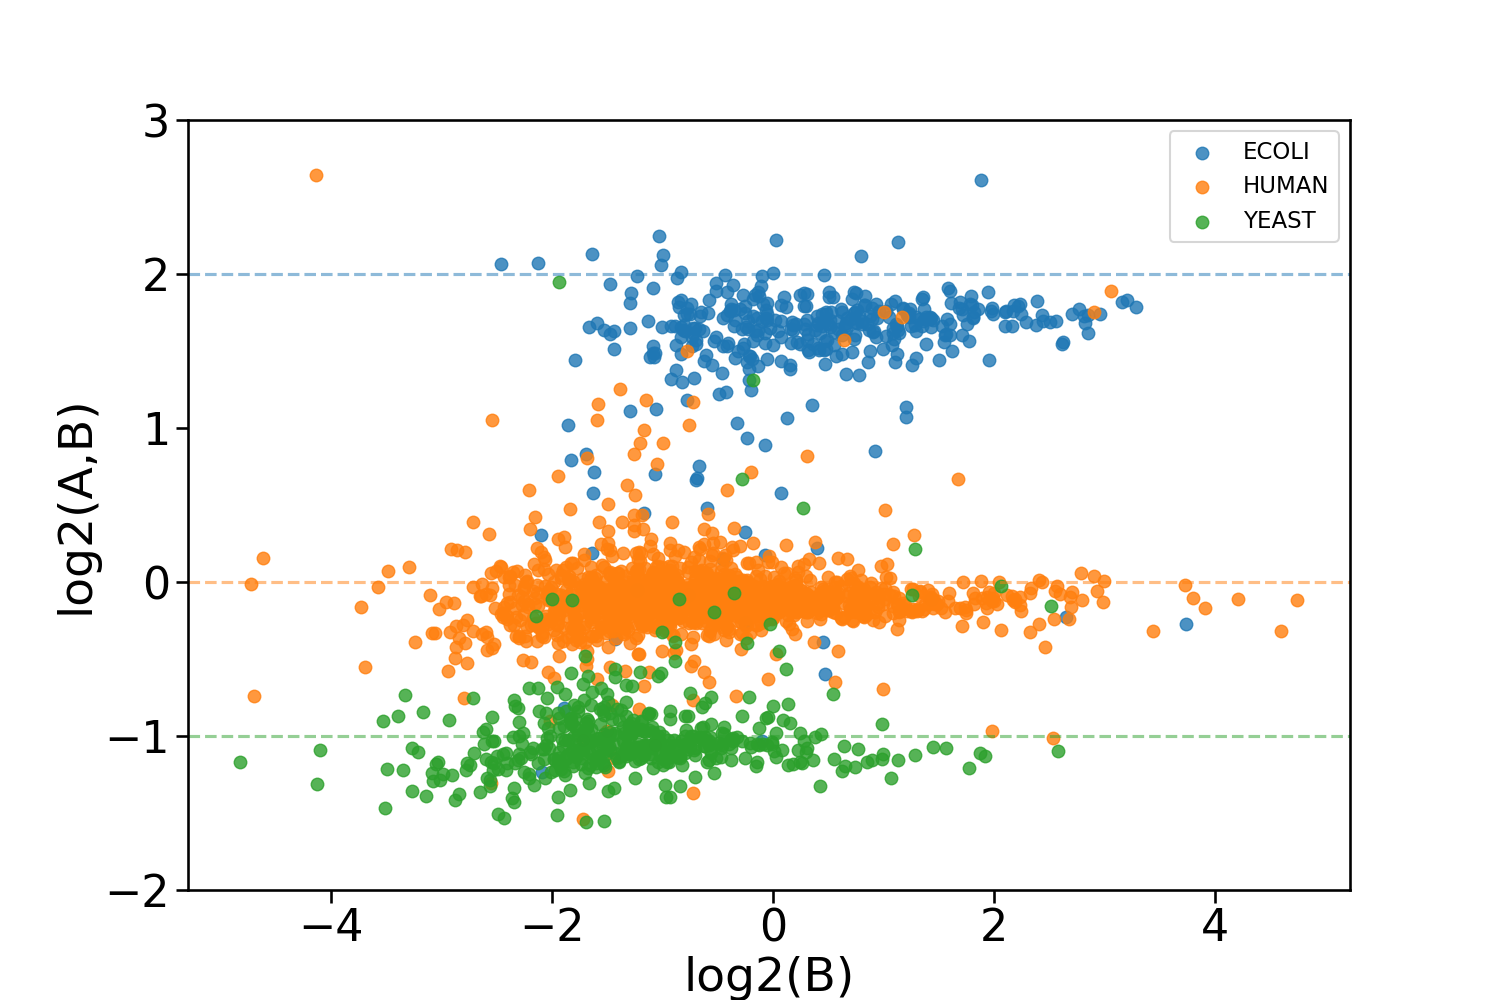
\includegraphics[width=0.45\linewidth]{../../result/report_plots_pipeline/scatter_ID_msqrob2.png} \\
        C & D 
    \end{tabular}
    \caption{{\bf Summarized protein fold changes as a function if abundance.} The distribution of estimated fold changes as a function of estimated abundance as reported through the (A) MAP estimates from Triqler, (B) Top3, (C) MSstats, and (D) MSqRob2.  As Triqler reports relative values for protein abundances the Triqler plot includes  Top3 reported protein abundances as a stand-in for the $log_2(B)$ values. The actual pipetted fold changes were indicated by a dashed line. See Supplementary Figure \ref{fig:fc_scatter_supplement} for protein-level results for both ID and PS workflows. \label{fig:fc_scatter}}
\end{figure}



\begin{figure}[hbt]
    \centering
    \begin{tabular}{cc}
	    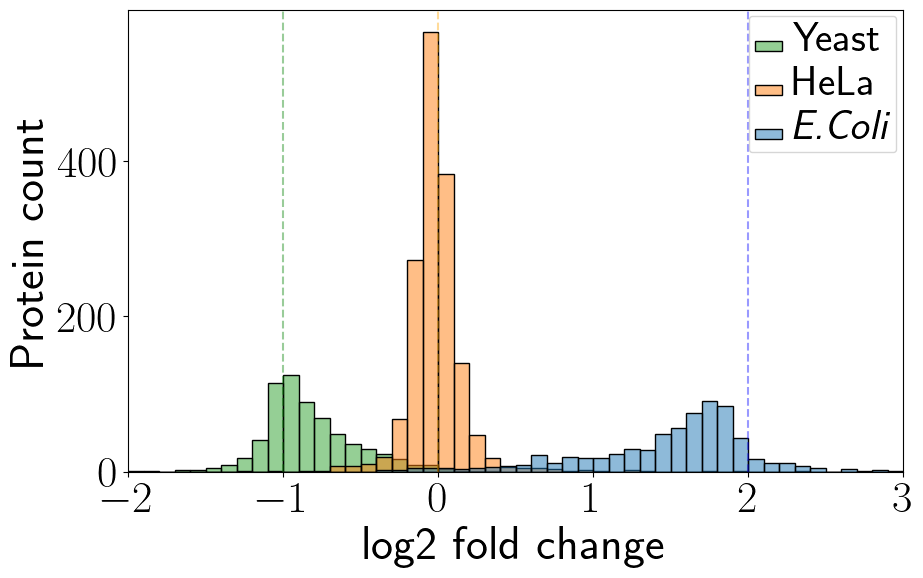
\includegraphics[width=0.4\linewidth]{../../result/report_plots_pipeline/histogram_ID_triqler.png} & 
	    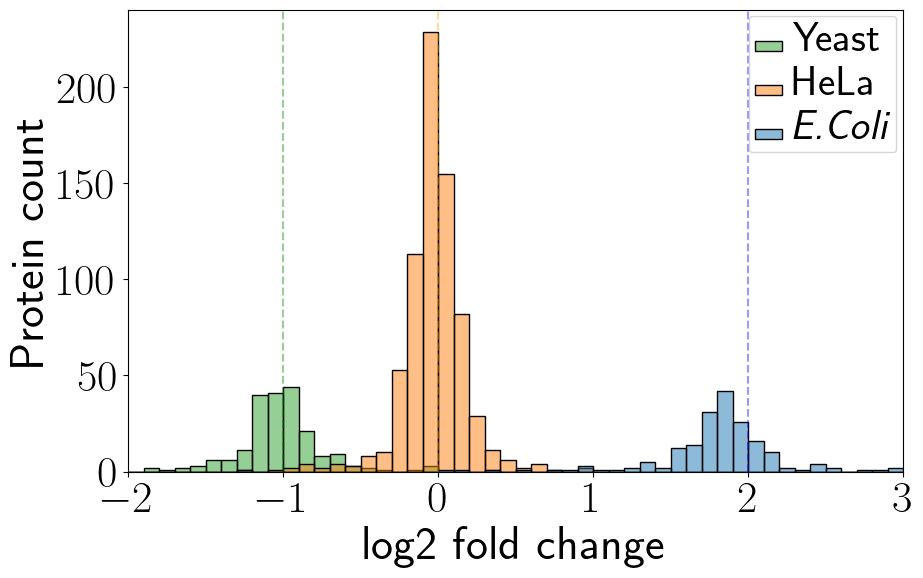
\includegraphics[width=0.4\linewidth]{../../result/report_plots_pipeline/histogram_ID_top3.png} \\ 
        A & B \\ 
	    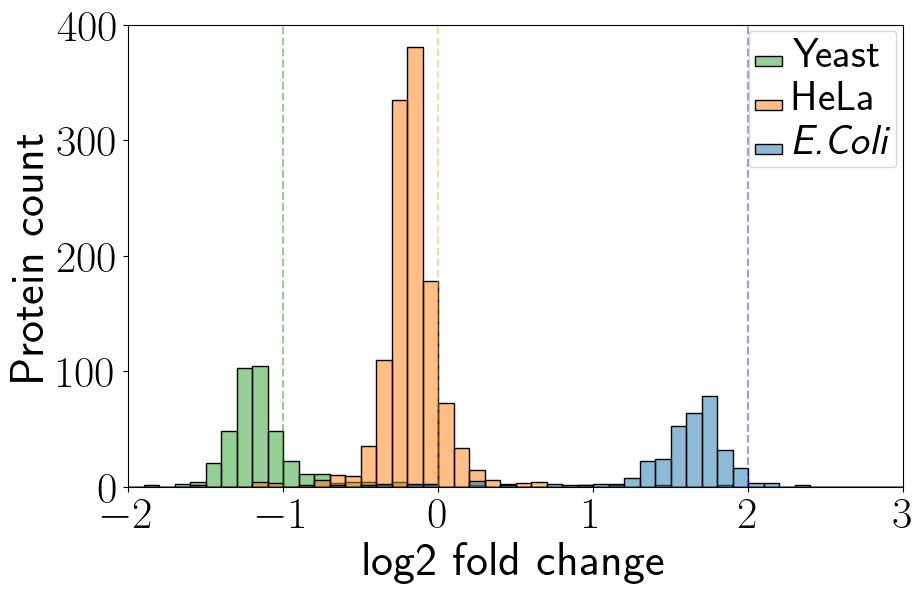
\includegraphics[width=0.4\linewidth]{../../result/report_plots_pipeline/histogram_ID_msstats.png} & 
	    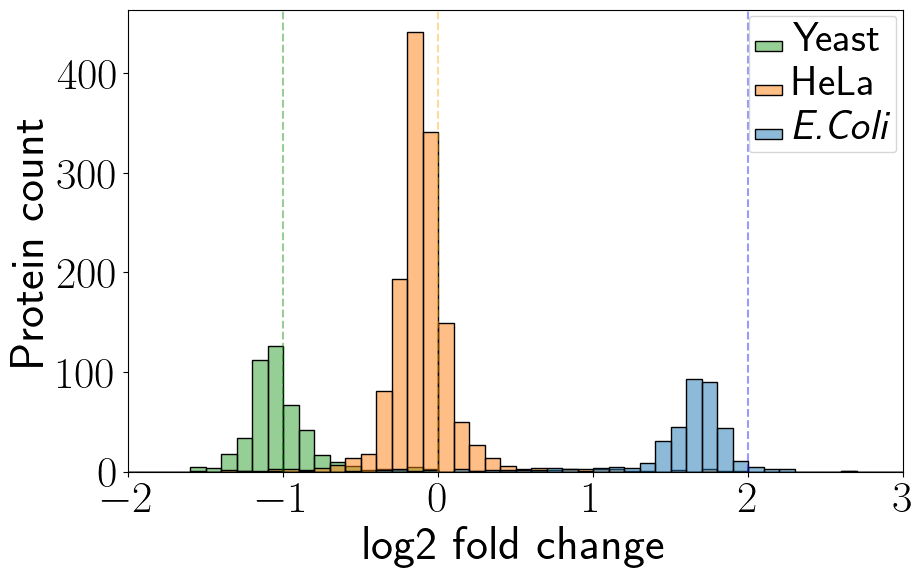
\includegraphics[width=0.4\linewidth]{../../result/report_plots_pipeline/histogram_ID_msqrob2.png} \\
        C & D 
    \end{tabular}
    \caption{{\bf Comparison of reported fold-change distributions.} We used protein data from the ID spectral library pipeline and (A) Triqler, (B) Top3, (C) MSstats, and (D) MSqRob2. The dashed lines indicate the pipetted log2-fold change ratio between a specie and HeLa samples. We noted that the empirical densities of the protein counts are less biased for Triqler and Top3 than MSstats and MSqRob2, as the apex of their distribution was found closer to the true fold-change difference (see Supplementary Figure \ref{fig:fc_histogram_supplement} for reported fold-change distributions for both ID and PS workflows). For these histograms, we included all the summarized proteins and did not remove any proteins based on  the significance or fold-change thresholds. \label{fig:fc_histogram}}
\end{figure}



\subsubsection*{Comparison of ability to discriminate differentially from equivalently abundant proteins}

As the first quantitative test of performance, we compared the methods' reported number of differentially abundant {\em E. Coli} and yeast proteins as a function of the number of HeLa proteins (Figure \ref{fig:diff_vs_hela}). As the former two lysates were injected in different concentrations and the HeLa was at constant concentration over the sample groups a higher number of non-HeLa proteins for a similar number of HeLa-proteins is seen as better performance.  Overall, it seems like Triqler reports more differentially abundant protein for every non-differentially abundant protein for both the peptide abundances generated by the ID spectral library and PS spectral library pipelines. The results can be found in Supplementary Figure \ref{fig:ability_to_differentiate_differentially_abundant_specie_vs_hela}. % Surprisingly, Top3 performs has more true differentially abundant proteins for every false protein than MSstats. 

\begin{figure}[hbt]
    \centering
    \begin{tabular}{lclc} 
        A & 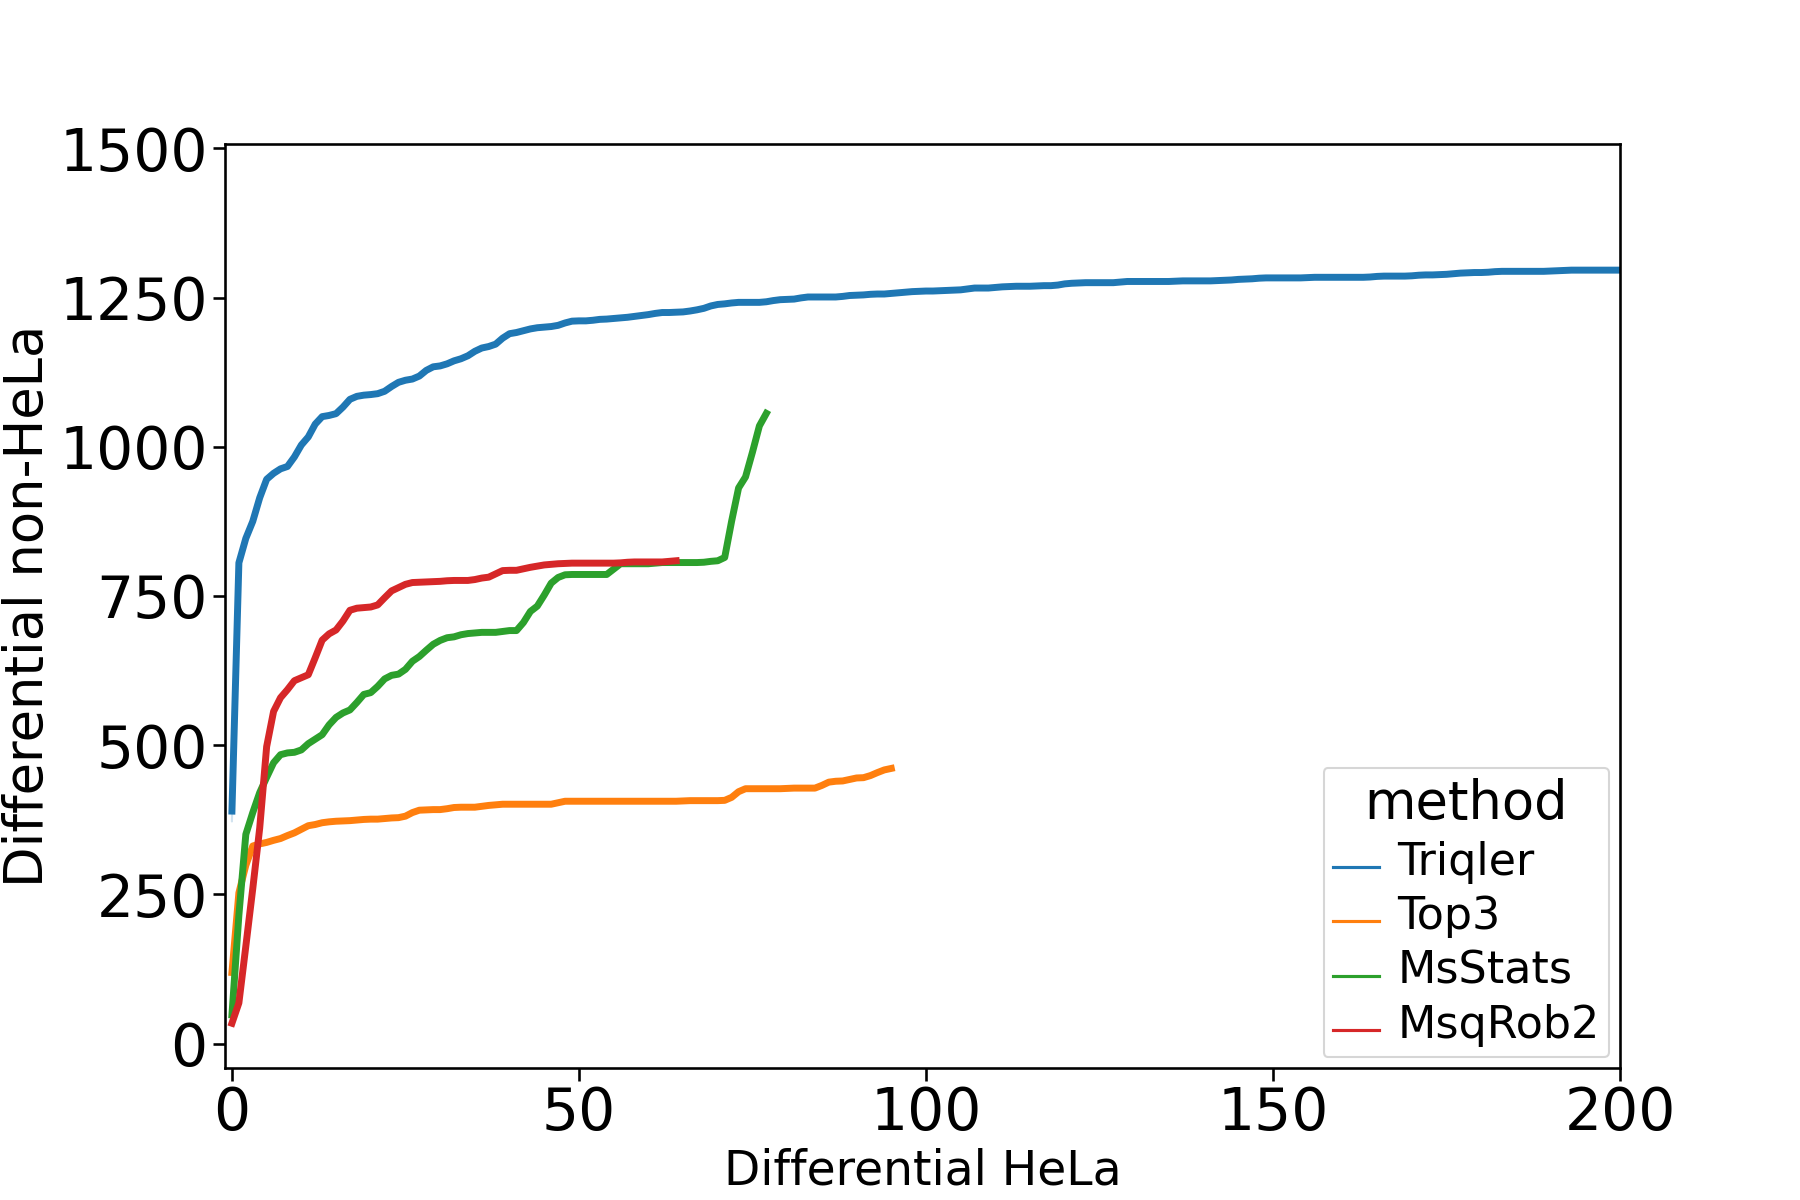
\includegraphics[width=0.45\linewidth]{../../result/report_plots_pipeline/diff_HeLa_vs_nonHeLa_ID_all_0.51.png} & 
        B & 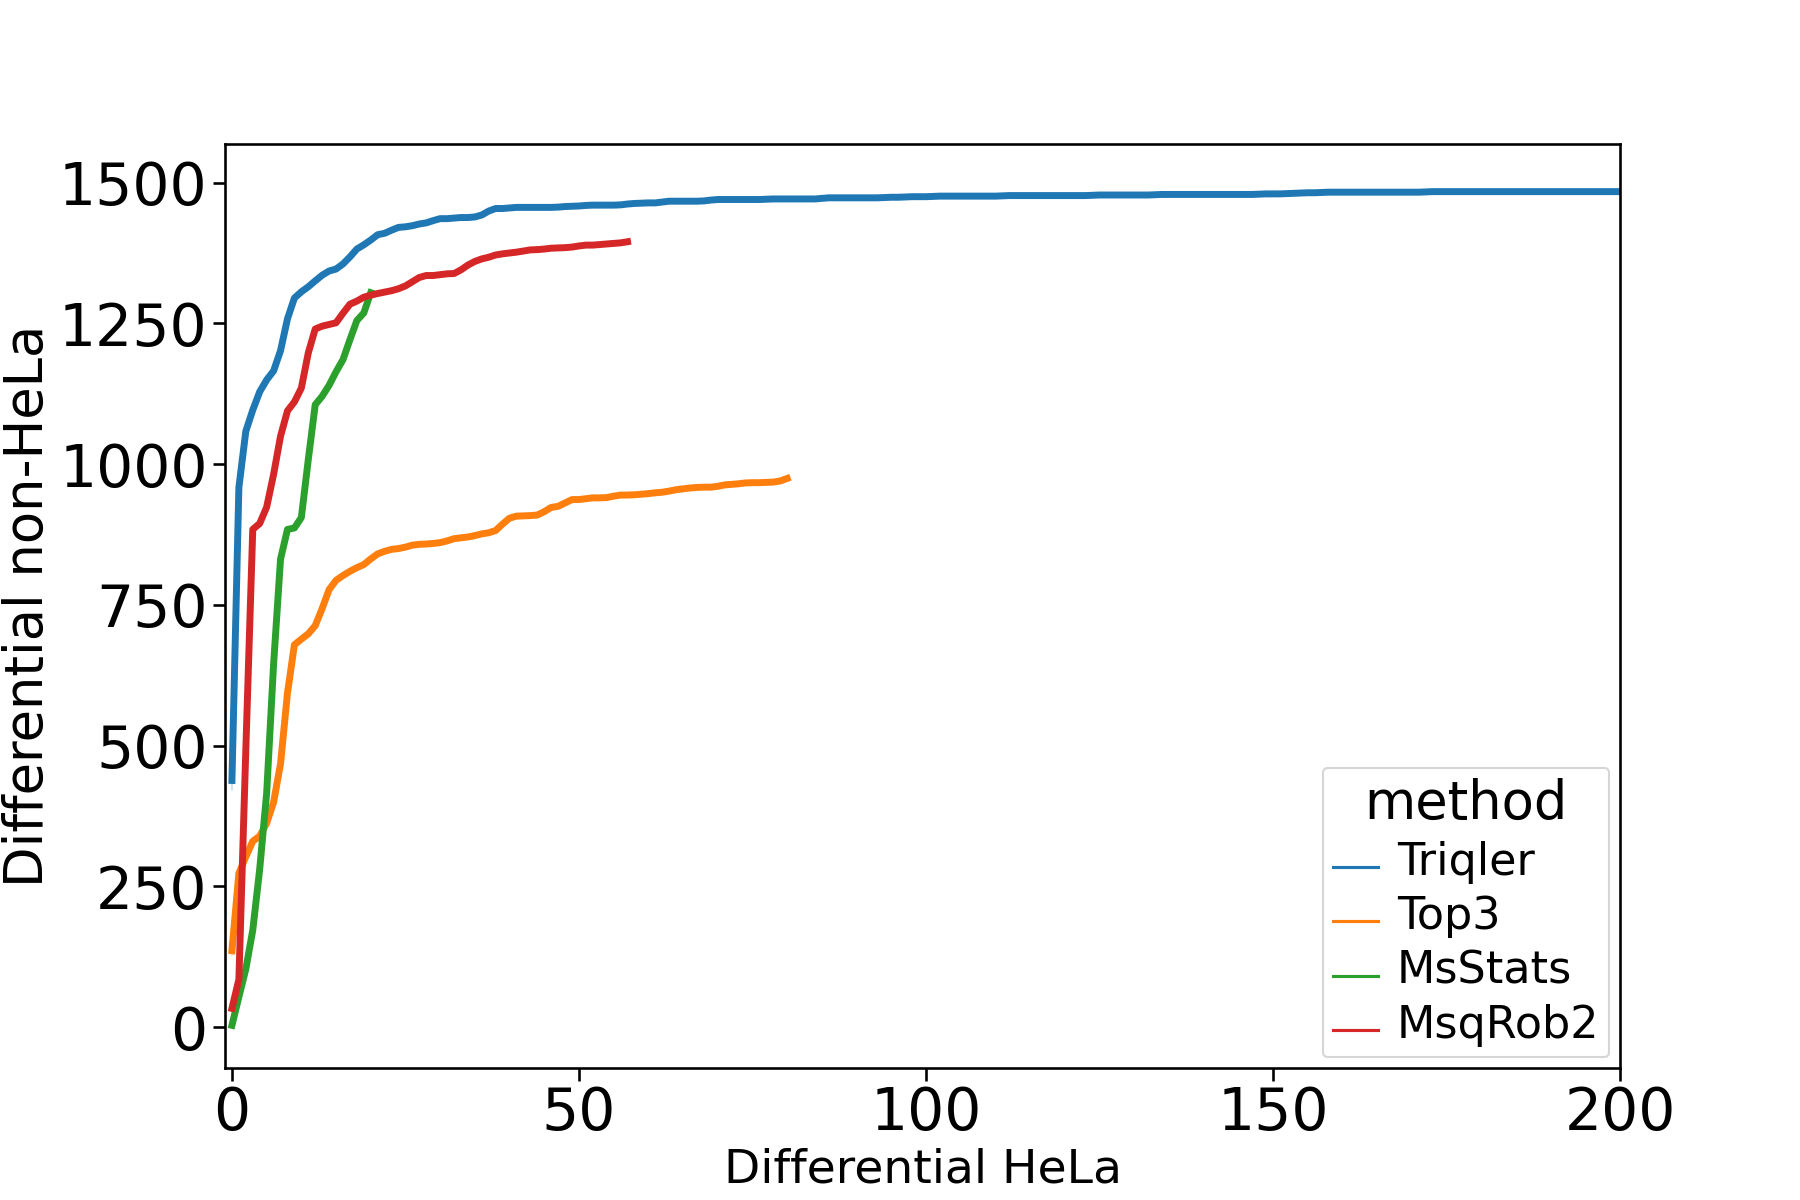
\includegraphics[width=0.45\linewidth]{../../result/report_plots_pipeline/diff_HeLa_vs_nonHeLa_PS_all_0.51.png} \\
    \end{tabular} 
    \caption{{\bf Comparison of ability to differentiate proteins with differential abundance between conditions} We plotted the number of reported differentially abundant  {\em E. Coli} and yeast proteins as a function of the number of proteins from the HeLa background when sorting according to significance for (A) ID pipeline and (B) PS pipeline. For the test, we selected a fold-change evaluation of 0.51 for Triqler and a fold-change threshold of 0.51 for Top3, MSstats and MSqRob2. All methods had an protein-level FDR-threshold of 0.01. (Supplement Figure \ref{fig:ability_to_differentiate_differentially_abundant_specie_vs_hela} shows differential abundance for each specie). \label{fig:diff_vs_hela}}
\end{figure}

\subsubsection*{Comparison of statistical calibration}

Further, we tested the statistical calibration of the summarization methods. We hence investigated the relationship between the fraction of wrongly reported differential abundant proteins (i.e. the fraction of HeLa proteins among all reported differential abundant proteins), and each inference method's estimated false discovery rate (See Figure \ref{fig:frac_hela_vs_fdr} and Figure \ref{fig:frac_hela_vs_fdr_supp}). Since the FDR is calculated for a specific dataset, we recalculate the FDR:s using q-value method after thresholding, so that the FDRs are recalibrated to the smaller data set. We observe that when we don't apply any fold-change threshold the calibration for MSstats, MSqRob2 and Top3 are bad, but they get better with a fold-change threshold. Triqler does not require any fold-change thresholding. We observe that Triqler is closer to the diagonal line (perfect calibration line) than the other methods and does not have a polynomial calibration curve as MSstats and MSqRob2 after applying the fold-change threshold. 

%We observed that Triqler, Top3, and MSqRob2 give estimates that are close to the true fold-change level than MSstats. This is somewhat surprising given that both MSstats and MSqRob2 are using the Benjamini-Hochberger corrections which are generally found more conservative than $q$~value estimates.

%We observed that Triqler and Top3 were reporting slightly more accurate estimates than MSstats and MSqRobSum. This is somewhat surprising given that both MSstats and MSqRobSum are using the Benjamini-Hochberger corrections which are generally found more conservative than $q$~value estimates.

\begin{figure}[hbt]
    \centering
    \begin{tabular}{cc} 
        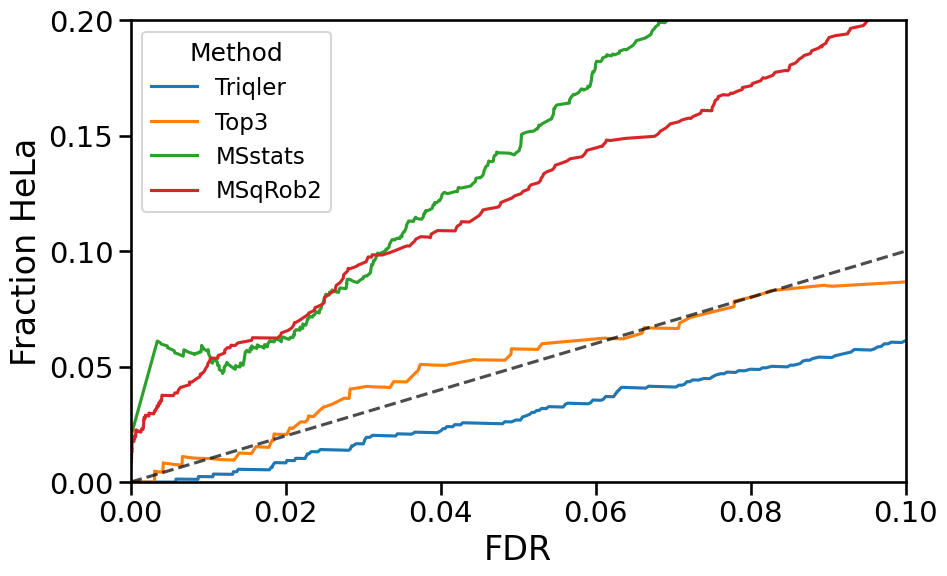
\includegraphics[width=0.5\linewidth]{../../result/report_plots_pipeline/calibration_ID_0.png} & 
        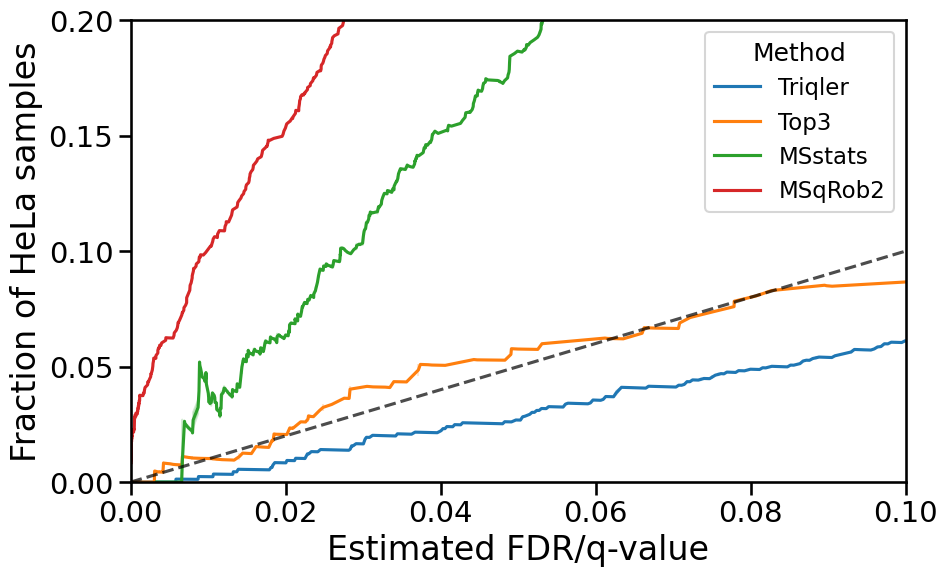
\includegraphics[width=0.5\linewidth]{../../result/report_plots_pipeline/calibration_ID_0.51.png} \\
        A & B
    \end{tabular}
  \caption{{\bf Comparison of calibration of the compared summarization methods.} We plotted the fraction of reported differentially abundant HeLa proteins as a function of $q$~value threshold for (A) non fold-change thresholded and (B) fold-change thresholded at 0.51, which is the lower bound computer by Triqler. The multiple test correction is performed with the $q$~value for Triqler and Top3, while Benjamini-Hochberger corrections were used for MSstats and MSqRob2. \label{fig:frac_hela_vs_fdr}}
\end{figure}

%\subsubsection*{Differential abundance reported by the protein quantification tools.}


%We also investigated the number of reported differential abundant proteins as reported by our four protein summarization methods. The results can be found in Supplementary Figure \ref{fig:ability_to_differentiate_differentially_abundant_specie_vs_hela}. Triqler reports the most differentially abundant proteins per .



\section*{Discussion}

Here we have shown that Triqler operates well for DIA data, despite originally intended for DDA data. We also find that Triqler outperforms other protein summarization methods on our engineered benchmark set, both in terms of sensitivity and accuracy in its error estimates. Triqler was also able to detect a higher number of differentially abundant proteins at a more accurately reported false discovery rate, than the compared methods. The absence of filtering and imputation steps before Triqler benefits the analysis by making it both more user-friendly by reducing parameter choices and inducing less bias into the result. 

The analytes in shotgun proteomics are peptides and not proteins or proteoforms. Nevertheless, most users of mass spectrometry use and will continue to find reasons to report findings on a protein level. It makes sense to put efforts into a better understanding of which protein inference tools to use at what occasion and how to summarize peptide abundances into protein relative concentration values.  Also, protein summarization gives lower variance than peptide-level analysis, and it reduces the number of hypotheses tested and reduced the number of missing values, which can have a major impact on the quality of the analysis \cite{plubell2021can}.   

One important remark is that the sequence database that we used for matching the spectra was filtered so that only one protein per peptide was kept, to control for any difference in protein inference strategies used by our compared protein summarization methods. There is currently no consensus on how to handle multiple proteoforms in bottom-up proteomics. Hence, we believe that protein inference strategies that can account for multiple proteoforms would greatly benefit the field by improving the quality of the quantitative analysis. 

We do see some differences in how DIA and DDA peptide-level abundance data appear. For instance, there are more missing values in the DDA than in the DIA data. However, we find that qualitatively the types of data are similar, at least in the sense that Triqler's underlying assumption of missing values seems to be as valid for DDA and DIA data.

It is therefore quite hard to evaluate how the performance of a data processing pipeline is influenced by its components. This should not stop the field from trying to establish the features of the different processing steps \cite{dufresne2014abrf,gatto2016testing,navarro2016multicenter}. Unbiased comparisons of software tools are challenging for several reasons \cite{dufresne2014abrf}. Methods can be assessed by scientists lacking relevant expertise, the tested methods may be lacking sufficient documentation and the interpretation of test results may be subjective \cite{yates2012toward,leprevost2014best,pak2013clustering,faircomparison2015}. By using the same data set we can assure that the data set is processed consistently and further the analysis by extending it to protein summarization procedures.

Lastly, we want to highlight the benefit and importance of datasets such as the one provided by Navarro et al. \cite{navarro2016multicenter}. These benchmarking datasets make it easy for the scientific community to investigate computational tools by providing a golden standard and significantly facilitating benchmark studies. 

\section*{Acknowledgements}


\section*{Funding}

This work was supported by grants from the Swedish Research Council (grant 2017-04030).

\section*{Supporting information}

\bibliographystyle{unsrt}
%\bibliography{benchmark}
\bibliography{benchmark.bib}
\end{document}



